\documentclass[10pt, french]{article}
\usepackage[square,numbers]{natbib}
\bibliographystyle{plainnat}

\usepackage[french]{babel}
\usepackage[T1]{fontenc}
\usepackage[utf8]{inputenc}

\usepackage{url}
\usepackage{hyperref}

\usepackage{amsmath}
\usepackage{amsfonts}
\usepackage{amssymb}

\usepackage{graphicx}
\usepackage{float}
\usepackage{lipsum}
\usepackage{multicol}
\usepackage{xcolor}

\usepackage[font=small]{caption}
\addtolength{\abovecaptionskip}{-3mm}
\addtolength{\textfloatsep}{-5mm}
\setlength\columnsep{20pt}

\usepackage[a4paper,left=2cm, right=2cm, top=2cm, bottom=2cm]{geometry}

\author{Benjamin Badouaille \qquad Eliott Camou \qquad Thomas Horrut}

\title{Mesure expérimentale de la quantité de données phonétiques nécessaire à un modèle
de langue ancienne pour une reconstruction non-supervisée de ses proto-formes}

\begin{document}
	\selectlanguage{french}
	\begin{center}
		{\Large \textbf{Mesure expérimentale de la quantité de données phonétiques nécessaire à un modèle de langue ancienne pour une reconstruction non-supervisée de ses proto-formes \footnote{Cet article scientifique relève de la fiction.}}}\\
		\vspace{2em}
		{\large Benjamin Badouaille$^2$ \qquad Eliott Camou$^2$ \qquad Thomas Horrut$^2$}\\
		\vspace{1em}
		\textit{$^2$Université de Bordeaux - 351 cours de la Libération CS10004, 33405 Talence     CEDEX}\\
            \vspace{1em}
            \today
	\end{center}

	\begin{center}
		\rule{150mm}{0.2mm}
	\end{center}

	\begin{abstract}
        Les derniers algorithmes d'apprentissage non supervisé que les chercheurs ont mis 
        au point pour la reconstruction des proto-formes nécessitent une grande quantité 
        de données phonétiques sur les langues descendantes, avec l'identification des cognats. 
        Cependant, ils ont également besoin d'une quantité de données sur la proto-langue 
        qui n'a pas été mesurée. La déterminer permettrait de vérifier si ces algorithmes 
        sont adaptés à l'étude de langues dont les ressources rassemblées par les linguistes 
        sont encore rares. Le but de cet article est de présenter une expérience qui réalise cette mesure. 
        Nous n'avons pas pu la réaliser avant la date limite. Néanmoins, nous avons émis quelques 
        hypothèses sur ses résultats.
        Notre méthode a consisté à former neuf modèles de langage au niveau 
        des caractères IPA et à exécuter un modèle de reconstruction avec chacun d'entre eux. 
        Nous comparons les résultats de chaque exécution avec la distance d'édition moyenne et pouvons conclure 
        sur les variations de pertinence en fonction de la quantité de données et 
        de l'architecture du modèle linguistique.\\

        \textbf{Mots-clés :} Reconstruction proto-formes, cognats, modèle de langue, n-gramme, résaux neuronaux récurrents, changement phonétique, apprentissage non-supervisée, Espérance-Maximisation, Monte-Carlo, chaîne de Markov.\\

        \vspace{2em}
        \begin{center}
            \textbf{Abstract}
        \end{center}
        
        The last unsupervised learning algorithms that researchers have developed for 
        proto-form reconstruction require a large amount of phonetic data about posterior 
        languages, with cognate identification. However, they also still need a 
        quantity of data about the proto-language which has not been measured. Determining it
        would allow to check if these algorithms are suitable to study languages for which resources 
        that linguists have gathered are still scarce. The aim of this article is to present an 
        experiment which realize that measure. We couldn't carry it out before the deadline. 
        Nonetheless, we have raised some hypothesis about its results.\\
        Our method was training nine IPA-character level language models and after executing a prior 
        reconstruction model with each of them. We compare the results of each execution with 
        the average edit-distance and can conclude about variations in relevancy according 
        to the data quantity and the language model architecture.\\

        \textbf{Keywords:} Proto-form reconstruction, cognates, language model, n-gram, recurrent neural networks, phonetic change, unsupervised learning, Expectation-Maximization, Monte-Carlo EM.
        
	\end{abstract}

	\begin{center}
		\rule{150mm}{0.2mm}
	\end{center}		

	\vspace{5mm}
	
\begin{multicols*}{2}

\renewcommand*\contentsname{Sommaire}
\tableofcontents

\section{Observation}
\subsection{La reconstruction de la proto-langue et son automatisation}
La linguistique historique a montré qu'un groupe d'idiomes peut être caractérisé 
par une langue ascendante commune. La conséquence principale est qu'un mot d'une 
langue ancienne a pu diverger en un ensemble de nouveaux mots, qu'on nomme des 
cognats, appartenant à différentes langues postérieures. Compte-tenu de ce 
phénomène-ci, la méthode comparative a émergée pour reconstruire dans une langue 
ancienne ses formes, c'est-à-dire ses mots à des accords grammaticaux près. 
En effet, la déduction d'une forme, qu'on qualifie de proto-forme, s'effectue à partir 
d'un ensemble identifié de cognats dont elle est supposée être l'ancêtre. 
La reconstruction est alors généralement menée par des linguistes, qui tâchent de s'accorder 
avec de nombreux principes, telles que les règles de variations phonétiques définies par 
la linguistique diachronique. Elle permet de constituer des lexiques pour la traduction de documents 
mais aussi de modéliser des langues à l'ancienneté toujours plus importante, la remontée ultime dans 
l'arbre généalogique des proto-langues étant l'indo-européen.\cite{campbell}

Ce procédé exige néanmoins un certain coût en temps et en connaissances, ce pourquoi des tentatives 
d'automatisation ont débuté dès les années 1970. \cite{bouchard}. La tâche informatique à réaliser 
ici s'inscrit dans de l'apprentissage machine déployé pour construire un modèle $f$ qui, à un ensemble 
de cognats $C=\{y_l : l \in L\}$ dans un ensemble de langues descendantes $L$, associe sa proto-forme 
ascendante $x$ ayant le plus probablement existée dans la proto-langue. Les éléments $x$ et $y_l$ sont 
représentés phonétiquement par des chaînes de caractères de l'Alphabet Phonétique International (IPA). 
L'entraînement du modèle s'effectue à partir d'une liste $D$ d'ensembles de cognats, constituée 
au préalable. Dans le cas d'un apprentissage supervisé, nous disposons également pour chaque ensemble 
de cognats $C_D$ de $D$ sa proto-forme vérifiée $x_C$.

Plusieurs approches sont fondées sur l'intervention interne de modèles plus élémentaires de prédiction 
des variations phonétiques (modèles d'édition) propre à chaque divergence entre une proto-langue ancêtre 
et une de ses descendantes. L'entraînement se réalise alors au niveau de ces modèles, qui sont caractérisés 
par des architectures tantôt statistiques et basées sur des propriétés admises par la linguistique 
diachronique\cite{bouchard}, parfois neuronales, avec l'apprentissage des règles de diachronie qui 
est dans ce cas attendue d'être faite par la machine\cite{andre}\cite{meloni}.

Les méthodes d'automatisation sont donc diverses. Toutefois, il est fréquent que leur évaluation 
se fasse expérimentalement sur de la prédiction de formes latines à partir de cognats dans les 
langues romanes modernes, le latin étant en effet une langue ancêtre dont de nombreuses ressources 
sont à portée pour mener des évaluations pointues des résultats prédits. \cite{andre}\cite{bouchard}\cite{meloni}

\subsection{L'intérêt de la démarche non-supervisée pour un problème à faibles ressources}
La question de la quantité de données nécessaires à l'entraînement des modèles est centrale, 
puisqu'on considère généralement la tâche de reconstruction des proto-formes comme un problème 
d'apprentissage à faible ressources. L'ordre de grandeur du nombre d'ensembles de cognats et 
de proto-formes qu'on pourrait se procurer à partir du travail des linguistes est en effet 
bien inférieur à celui du nombre d'entrées que les dernières technologies d'apprentissage 
automatique en Traitement Automatisé du Langage ont l'habitude de recevoir pour faire des 
prédictions avec précision.\cite{fourier}\\
Une tâche informatisée idéalement généralisée de reconstruction devrait d'autant plus ne 
requérir qu'un minimum de données sur la proto-langue, pour le cas où l'on souhaite l'appliquer 
à des langues éteintes dont on dipose ne dispose que de peu de connaissances.

Par conséquent, la faible taille du corpus d'entraînement contraint d'une part les chercheurs à 
limiter les complexités architecturales des modèles d'édition, en restant par exemple sur un 
nombre mince de couches de réseaux de neurones récurrents (RNN), dans le cas des 
démarches neuronales.\cite{andre}\cite{meloni} Ce fait sera réabordé dans la section 3 pour 
justifier quelques hypothèses.

Enfin, l'option d'un apprentissage non-supervisé offre l'avantage d'avoir besoin de bien 
moins de mots phonétiques de la proto-langue établis par les linguistes. En théorie, même 
aucune reconstruction correcte ne devrait être à fournir, mais la prochaine section montrera 
qu'en pratique une certaine quantité de proto-formes reconstruites correctement demeure nécessaire.


\subsection{L'état de l'art de la démarche neuronale dans la prédiction de proto-formes}
Dans l'état actuel de nos connaissances, la dernière approche non-supervisée en date est 
celle de Andre He et al. Elle consiste à entraîner des modèles neuronaux d'édition tout en 
modifiant de manière itérative les proto-formes associées à des ensembles de cognats, à 
travers la répétition d'un algorithme probabiliste d'espérance-maximisation (EM) 
de type Monte-Carlo.\\
La richesse de la liste d'ensemble de cognats a de l'importance dans la précision du modèle 
entraîné puisque des calculs de paramètres d'entraînement sont fondés sur des moyennes de probabilités 
calculées pour chaque ensemble de cognats.


Les résultats de cette dernière approche ont surpassé ceux sortis par de précédents modèles à la stratégie 
similaire, la comparaison s'étant effectuée en termes de distance d'édition entre les proto-formes latines 
prédites et les proto-formes reconstruites réelles. L'innovation s'est faite avec le choix d'une architecture 
neuronale récurrente (Long-Short Term Memory ; LSTM) pour les modèles d'édition. Toutefois, 
aucune étude documentée des règles de changement phonétique apprises par ces réseaux neuronaux 
n'a encore été entamée.\cite{andre}

\section{Problématique}

L'apprentissage proposé précédemment n'a cependant pas su se passer de l'intervention d'un modèle bi-gram de langue du latin pour le calcul de probabilités nécessaires à l'étape d'échantillonnage de la EM. Les chercheurs le justifient par le bruit présent dans le corpus des cognats des langues romanes.\cite{andre} Ce modèle renvoie la probabilité $p(x)$ qu'une chaîne $x$ de caractères de l'IPA puisse représenter un mot appartenant à cette langue, et nécessite une liste de mots y appartenant réellement pour être entraîné, en identifiant des structures au voisinage de chaque caractère phonétique, cette identification s'effectuant selon son architecture.\cite{jurafsky_ngram} L'approche étudiée ici requiert donc des connaissances préliminaires sur la proto-langue à reconstruire. L'ambition de cet article est d'en déterminer un ordre de grandeur de manière expérimentale.

\section{Hypothèses}

Soit $|D_{\text{ML}}|_i$ la taille du corpus d'entraînement d'un modèle de langue $i$ de la proto-langue.
Il est supposé que, pour chaque architecture $i$ de modèle de langue exploitable dans une configuration fixée de l'algorithme de EM proposé par Andre He et al., il existe des tailles intrinsèques de corpus d'entraînement $a_i$ et $b_i$  ($a_i<b_i$) telles que :
\begin{itemize}
    \item Pour $|D_{\text{ML}}|_i$ variant en dessous de $a_i$, les reconstructions finalement prédites ont une pertinence trop faible.
    \item Pour $|D_{\text{ML}}|_i$ augmentant dans $[a_i; b_i]$, la pertinence des résultats prédits croît de manière non-négligeable.
    \item Pour $|D_{\text{ML}}|_i$ variant au-delà de $b_i$, la pertinence ne croît plus que de manière asymptotique, en restant en-dessous d'un niveau limite. 
\end{itemize}
Dans le cas d'une vérification de cette hypothèse variationelle, est aussi proposée l'intuition que, si une architecture $i$ de modèle de langue est plus complexe qu'une architecture $j$, alors :
\begin{itemize}
    \item $a_i \leq a_j$
    \item $b_i \leq b_j$
    \item La pertinence maximale est plus importante avec le modèle $j$ que le modèle $i$.
\end{itemize}
L'hypothèse générale peut être résumée par le figuré \ref{fig:fighyp}.

\begin{figure*}[ht]
  \centering
  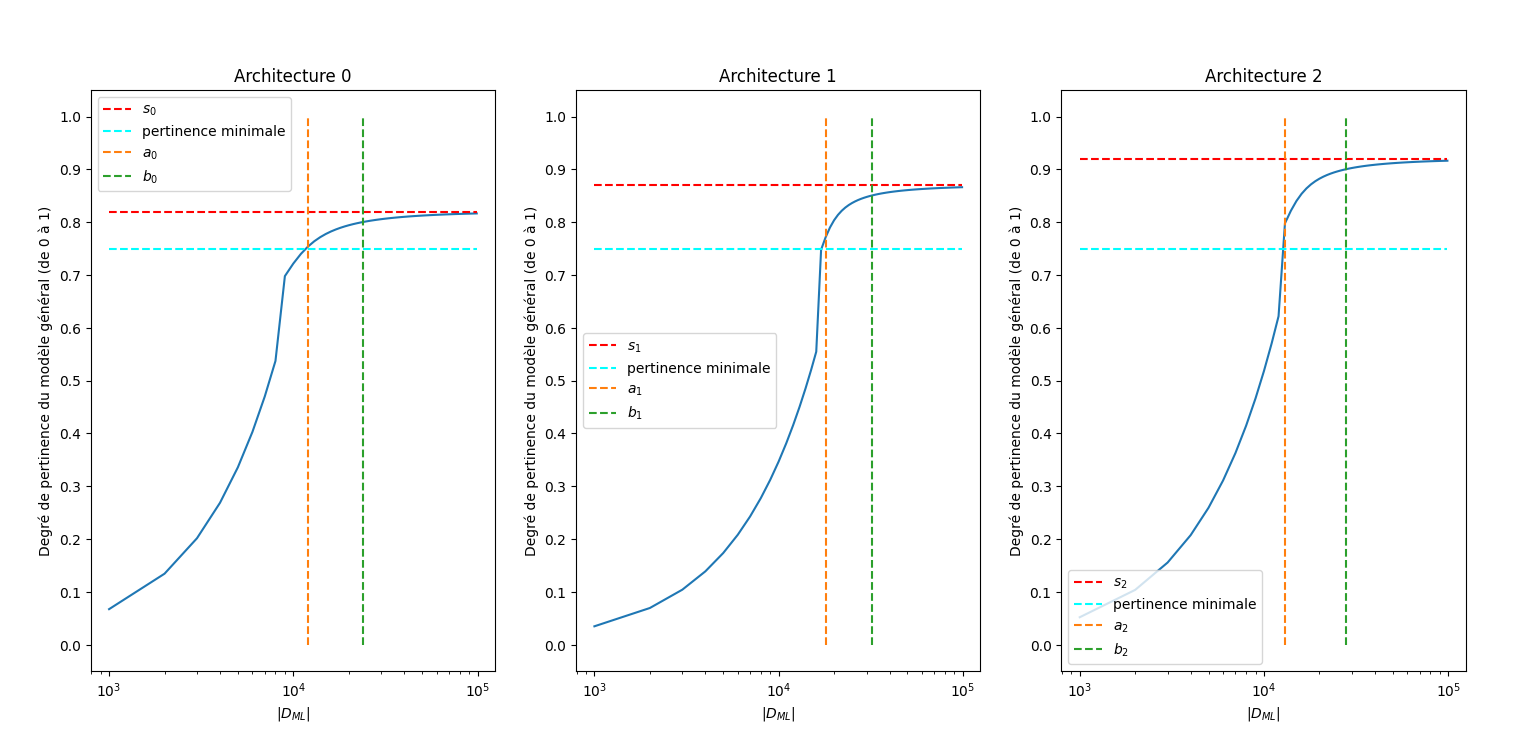
\includegraphics[width=\textwidth]{Figure_hyp.png}
  \caption{Courbes possibles d'évolution du degré de pertinence des modèles de reconstruction 
  en fonction de la quantité de données fournies au modèle de langue, si les hypothèses 
  variationnelles énoncées plus tôt sont validées. En échelonnant cette grandeur de 0 à 1, on définit 
  une pertinence minimale en-dessous de laquelle le modèle n'est certainement pas exploitable. 
  Les valeurs atteintes pour $a_i$ et $b_i$ sont attendues d'être différentes pour des 
  architectures différentes.}
  \label{fig:fighyp}
\end{figure*}

\section{Expérience}
\subsection{Comparaison des distances d'édition}
Pour mesurer l'impact du modèle de langue sur les performances du modèle de reconstruction, la distance d'édition a été utilisée. Elle quantifie l'écart entre deux séquences de caractères, en comptabilisant le nombre minimal d'opérations nécessaires (substitution, insertion ou suppression) pour passer de la première chaîne de caractères à la seconde. Dans le cadre de cette étude, l'écart entre la proto-forme latine produite par le modèle de reconstruction et celle de référence incluse dans la base de données de Meloni et al. (2021)\cite{meloni} sera mesuré. Cette mesure sera ensuite moyennée sur l'ensemble de la base de données, en fonction du modèle de langue utilisé et de sa quantité d'entraînement. D'une manière analogue à celle d'Andre He et al., ces moyennes seront accompagnées des écarts-types afin d'établir des incertitudes.\\
Pour chaque architecture de modèle de langue décrite, l'étude a consisté à entraîner le modèle sur un corpus de mots latins phonétisés au nombre (différent de celui de l'évaluation pour éviter les biais) de 10 000, puis de 15 000 et enfin de 20 000. À chaque augmentation de la taille du corpus, le modèle a été évalué en calculant la moyenne de la distance d'édition produite par l'écart entre la proto-forme prédite par le modèle de reconstruction et la proto-forme latine trouvée par les linguistes.

\subsection{Mise en place du modèle de reconstruction}
Les travaux de Andre He et al. (2022)\cite{andre} ont été pris comme référence pour notre étude. Leur papier propose un modèle d'édition et un entraînement suivant l'algorithme de Monte Carlo d'espérance maximisation, pour la reconstruction de proto-formes latines à partir d'un corpus d'ensembles de cognats préalablement identifiés dans les langues romanes qui sont l'Italien, le Français, l'Espagnol, le Portugais, et le Roumain. Leur modèle d'édition a été repris avec les mêmes paramètres, et a été configuré de la même façon. Concrètement, le modèle a été initialisé, comme suggéré dans leur papier, avant sa première maximisation, avec des échantillons provenant d'un modèle de chez Bouchard-Côté et al. (2009)\cite{bouchard}, qui a été entraîné pendant trois itérations EM. De même, le modèle d'édition a été volontairement sous-entraîné à l'étape de maximisation en fixant le nombre d'époques à 5. Et le nombre d'itérations EM effectué a été fixé à 10. Enfin, dans la reproduction de leur expérience, la même base de données a été utilisée, provenant de la révision de Meloni et al. (2021)\cite{meloni}, qui comprend des ensembles de cognats dans les langues romanes (cités) transcrits dans leur représentation IPA avec leur proto-forme latine produite par des linguistes. Cette base de données a servi à entraîner le modèle de reconstruction et à l'évaluer.

\subsection{Modèles de langue}
Pour tester notre hypothèse, trois architectures de modèles de langue ont été sélectionnées, 
qu'on énonce par ordre de complexité croissante : l'architecture bi-gramme, tri-gramme, puis 
le réseau de neurones récurrent. Pour chacune d'elles, trois modèles ont été entraînés avec un des corpus 
corpus latins décrits dans la sous-section suivante. 

\subsubsection{Base de données}
Pour entraîner ces modèles de langues, nous avons utilisé une base de données modifiée du CC-100 Web Crawl de 
chez Hugging Face\footnote{ https://huggingface.co/datasets/pstroe/cc100-latin}. Les modifications apportées 
ont été la suppression des \og pseudo-latins\fg (comme \og Lorem ipsum\fg), la séparation et la normalisation 
des mots avec la librairie Python CLTK\footnote{http://cltk.org/}, la conservation des lignes de textes 
uniquement contenant des lettres de l'alphabet latin, des chiffres, certaines ponctuations, et enfin la déduplication du corpus. Pour notre expérience, des modifications supplémentaires ont été apportées pour ne retenir que les lignes de textes contenant uniquement des lettres latines. Il est enfin vérifié que les mots latins dans ces lignes n'apparaissent jamais dans la base de données de Meloni et al. (2021). Enfin, chaque mot a été phonétisée grâce à la librairie espeak\footnote{https://github.com/espeak-ng/espeak-ng} afin d'entraîner des modèles de langue phonétique. Nous sommes en effet restés fidèles à la démarche principale qui était de travailler en assumant la transformation du mot ancêtre vers son descendant comme un processus génératif de modifications phonétiques \cite{andre}. Il a été vérifié que l'inventaire des caractères IPA apparaissant dans la base de données de Meloni et al. (2021)\cite{meloni}, noté $\Sigma'$, soit inclus dans l'inventaire de notre base de données phonétique, noté $\Sigma$. Ainsi, il est évité à l'étape de reconstruction de devoir travailler avec des caractères que le modèle de langue n'aurait jamais vus, ceci esquivant le passage d'un lissage à nos modèles de langues. 
Au vue de la taille du vocabulaire $\Sigma$ qui est relativement petite, inférieur à 50, chaque caractère de chaque mot de notre base de données phonétique a été encodé de façon 1 parmi n (ou plus communément nommé en anglais \textit{one-hot encoding}), où chacune des séquences de caractères (mots) vectorisées a été remplie de 0 pour convenir à la dimension d'entrée de nos modèles de langue.

\subsubsection{Implémentation des modèles et leur entraînement}
Le modèle bi-gramme a été construit en utilisant les probabilités conditionnelles estimées à partir de notre corpus de données. Pour se faire, toutes les paires de mots adjacentes dans notre base de données phonétiques ont été extraites, et la probabilité conditionnelle $P(w_i|w_{i-1})$ qu'un caractère de l'IPA $w_i$ apparaisse à la suite du caractère précédent $w_{i-1}$ a été calculée en divisant le nombre d'apparitions de la paire $(w_{i-1},w_i)$ par le nombre d'apparition du mot $w_{i-1}$ dans notre base de données. Ces probabilités conditionnelles sont ensuite stockées dans une matrice, où chaque ligne représente le caractère précédent et chaque colonne représente le caractère courant.\\
\indent L'implémentation du modèle tri-gramme suit un processus analogue à celui du modèle bi-gramme, mais cette fois-ci sont extraits des triplets de caractères IPA de notre corpus de données, et la probabilité conditionnelle $P(w_i|w_{i-2},w_{i-1})$ pour chaque triplet de caractères $(w_{i-2},w_{i-1},w_i)$ est calculée. La matrice finale de notre tri-gramme stocke les probabilités conditionnelles, avec chaque ligne qui représente les deux caractères précédents et chaque colonne qui représente le caractère courant.
Enfin, un modèle de réseaux de neurones récurrent (RNN) a été implémenté (Annexe A).\\
\indent Contrairement aux modèles de n-gramme qui ne considèrent que les $n-1$ caractères précédents 
pour estimer la probabilité du caractère courant, les RNN prennent en compte tous les caractères précédents 
pour estimer la probabilité du caractère courant. Les cellules (neurones) utilisées pour notre modèle sont 
des LSTM bidirectionnel. Le modèle prend en entrée une séquence de caractère et utilise une couche d'embedding 
pour convertir chaque caractère en un vecteur dense de nombres réels. Il a été entraîné avec l'algorithme 
d'optimisation de la descente de gradient stochastique (SGD) pour minimiser l'erreur de prédiction de 
chaque caractère dans un mot donnée.

\section{Résultats}

N'ayant pu faire fonctionner nos modèles de langues dans les délais impartis, nous dressons une liste des différents résultats possibles : 

\begin{enumerate}
    \item La distance d'édition est à peu près constante, quelque soit le modèle de langue et la quantité de données fournies pour son entraînement.
    \item La distance d'édition varie suivant l'architecture mais pas suivant la quantité de données. Elle diminue quand la complexité de l'architecture augmente, ou inversement.
    \item La distance d'édition varie suivant la quantité de données, mais cette évolution est à peu près équivalente à travers les types d'architecture. Elle diminue quand la quantité de données augmente, ou inversement.
    \item La distance d'édition varie suivant la quantité de données et l'architecture du modèle de langue.\ref{fig:figres}
\end{enumerate}

\noindent\textit{Les incertitudes auraient été obtenus en prenant l'écart type des distances d'édition obetnus pour calculer nos moyennes.}

\begin{figure*}[ht]
  \centering
  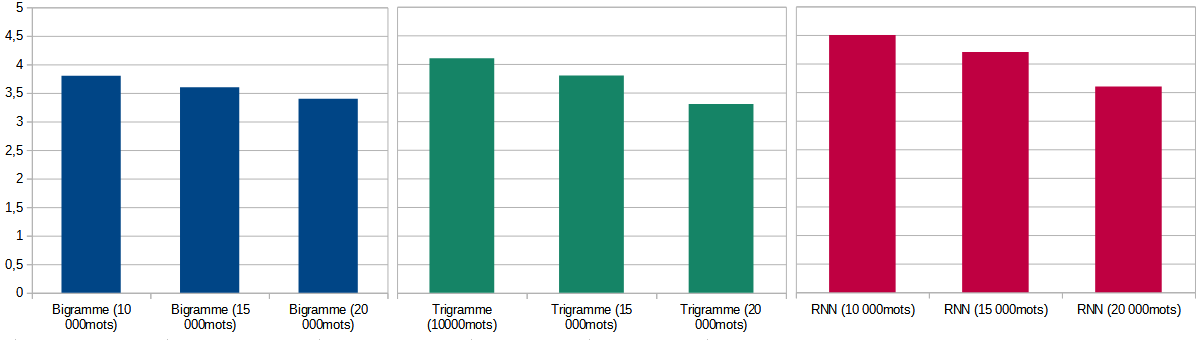
\includegraphics[width=\textwidth]{edit_distance_by_model.png}
  \caption{\textbf{Histogramme fictif} : Distance d'édition suivant le type de modèle et la quantité de mots latins phonétisés fournie. Résultat représentant le cas n°4 : la distance d'édition diminue au fil de la quantités de mots augmentent, quel que soit l'architecture. Cependant plus l'architecture se complexifie, plus la distance d'édition augmente.}
  \label{fig:figres}
\end{figure*}


\section{Interprétation}

\begin{enumerate}
    \item Si la distance d'édition ne bouge pas, peu importe le modèle de langue utilisé, même lors de l'ajout d'un grand nombre de données, alors cela démontre que le modèle de langue n'a pas de réelle influence sur le modèle de reconstruction. Nous pouvons en déduire qu'il n'est pas nécessaire de complexifier le modèle de langue, ni au niveau de son architecture, ni au niveau de son entraînement, la quantité de données sur la proto-langue étant alors peu importante au-delà d'un ordre de grandeur minimal. Ainsi, nous pouvons comprendre que le modèle de reconstruction a juste besoin d'un modèle de langue \og basique\fg pour s'orienter dans sa génération de proto-formes. À noter que la complexification d'un modèle de langue implique le besoin d'une plus grande quantité de données pour entraîner le modèle, ce qui n'est pas raisonnable face à la tâche de reconstruction d'une proto-langue, dont nous possédons souvent peu de données.
    \item Si la distance d'édition change uniquement suivant le type d'architecture du modèle de langue, mais pas suivant la quantité de données fournies (autrement dit, la distance d'édition reste constante pour chaque type de modèle, mais cette constante varie suivant le modèle), alors nous pouvons en déduire que le facteur limitant dans ce cas est le modèle de langue et non nécessairement la quantité de données. Il se peut néanmoins que nous n'ayons pas non-plus fait varier suffisamment cette quantité pour observer un écart important, sortant de nos écarts-type. Dans le cas où la distance d'édition diminue au fur et à mesure que le modèle de langue se complexifie, nous pouvons penser que le modèle de langue capture une meilleur représentation de la proto-langue ce qui permet au modèle de reconstruction d'être mieux guidé dans sa prédiction de proto-formes. Dans le cas inverse, nous pouvons comprendre qu'une capture plus complexe de la structure de la proto-langue se comporte comme un frein pour l'apprentissage du modèle de reconstruction.
    \item Si la distance d'édition varie uniquement en fonction de la quantité de données, nous pouvons alors choisir un modèle de langue simple à entraîner, comme le bi-gramme, et s'exempter de modèles de langue complexes qui n'apporteront rien de plus, même s'ils promettent de capturer des généralisations plus sophistiquées sur la proto-langue. Dans la situation où la distance d'édition diminue en fonction de l'augmentation de la quantité de données, cela peut traduire que le modèle de langue a capturé des structure de langue plus diverses (pas forcément plus complexe) permettant au modèle de reconstruction d'accéder à un inventaire plus grand pour effectuer les modifications sur les cognats modernes. Au contraire, si la distance d'édition augmente suivant la quantité de données, alors nous pouvons penser que la diversification du modèle de langue génère du bruit pour le modèle de reconstruction. 
    \item Si la distance d'édition varie suivant ces deux paramètres que sont l'architecture et la quantité de données, alors il devient plus difficile de conclure sur ces résultats. Cependant, si nous pouvons remarqué une tendance, comme le montre la figure \ref{fig:figres}, alors nous pouvons en déduire certaines propriétés. Dans ce dernier cas, qui contredit l'hypothèse que la distance d'édition diminue au fur et à mesure que le modèle se complexifie et que la quantité de données augmente, nous pouvons comprendre que le modèle de reconstruction ne s'éloigne pas de la règle que, si son modèle de langue est plus complexe, il a besoin de plus de données pour être performant. Cependant, rien ne nous permet d'affirmer qu'un modèle de langue plus complexe puisse apporter des performances meilleures pour une quantité assez importante de données fournies, face à des modèles de langues plus simples.
\end{enumerate}

\section{Conclusion et Limitations}
L'objectif principal des interprétations de cette expérience est d'engager une discussion sur la portée des démarches non supervisées dans l'état actuel de l'art pour la reconstruction de langues anciennes plutôt que que de déterminer de manière généralisée la quantité minimale de données linguistiques anciennes requises pour effectuer une reconstruction fiable par la machine.

Une première limite expérimentale évidente aura été celle de ne se pencher que sur une reconstruction concernant les langues romanes. Des expérimentations de reconstructions impliquant un arbre phylogénétique de langues à la structure bien différente ont eu lieu lors de travaux ultérieures, comme ceux de 2013 de Bouchard-Côté et al.\cite{bouchard_austro}. Leur modèle, en se penchant sur les langues austronésiennes\cite{greenville}, n'a en effet pas pu être surpassé par celui d'Andre He et al. \cite{andre}

Ensuite, nous avons veillé à conserver un maximum de paramètres expérimentaux définis par l'article auquel nous nous sommes référés. Il n'est pourtant pas exclu que quelques-uns de ces paramètres, dont notamment le nombre d'itérations de EM, que nous avons fixé à 10, aient influencé les résultats obtenus de manière non-négligeable. Effecuter des comparaisons à travers plusieurs valeurs de ces paramètres pourrait donc apporter des éléments plus riches pour traiter du sujet de cet article.

Enfin, comme évoqué dans l'interprétation, il se peut que la quantité de données que nous avons fait varier n'est pas suffisante entrainant des résultats non pertinents. Il est possible qu'il existe (ou non) un seuil de données à partir du quel la distance d'édition varie fortement, soit dans la continuité de sa tendance ou soit au contraire de sa tendance. 

\clearpage

\bibliography{biblio}
\pagebreak
\appendix

\section{Configurations et hyperparamètres pour le modèle de langue RNN}
\begin{itemize}
    \item Nombre de couches cachées : 1.
    \item Taille de la couche cachée : 50 neurones.
    \item Type de cellule RNN : LSTM bidirectionnelles.
    \item Fonction d'activation : La fonction ReLU utilisée pour la couche cachée, et  la fonction softmax pour la couche de sortie.
    \item Taux d'apprentissage : 0,001.
    \item Epochs : 100 epochs.
    \item Batch size : 32.
\end{itemize}

\end{multicols*}
	
\end{document}